\documentclass{article}
\usepackage{indentfirst, amsmath, amssymb, graphicx, tikz}
\usepackage[margin=1in]{geometry}
\usepackage{titlesec}
\usepackage[export]{adjustbox}
\usepackage{float}
\usetikzlibrary{positioning}
\titleformat{\section}{\normalfont\Large\bfseries}{\thesection}{1em}{}

\title{Rediscovering the Euclidean Algorithm \\
\large From Embodied Group-Splitting to Abstract Recursion}
\author{Mr. Stephen Chong}
\date{25 July 2025}

\begin{document}

\maketitle

\section*{Abstract}
This paper explores a plausible, stepwise cognitive and material pathway to the discovery of the Euclidean algorithm by framing division as a process that begins with naive groupings of material quantities—such as pebbles, tiles, or rope—and gradually evolves into recursive subdivision. Through a sequence of regularity-driven observations, this process converges toward a minimal and recursive pattern that leads naturally to the Euclidean algorithm. While the specific cognitive and material steps presented here are speculative, they are grounded in historically plausible practices, perceptual behaviors, and known mathematical developments of the ancient world. No direct historical evidence survives detailing the exact discovery of the Euclidean algorithm, but this paper consolidates a set of plausible intuitions and tactile strategies that may have seeded the recursive behavior we now recognize as the Euclidean algorithm.


\section{Embodied Origins of the Euclidean Algorithm}
Before the Euclidean algorithm was formalized as a mathematical procedure, its core behavior likely emerged from physical experience: splitting tangible quantities into equal-sized groupings—a behavior grounded in perception and material constraints. Ancient builders, surveyors, or stewards distributing goods would have often faced the challenge of dividing one length, pile, or batch into smaller, equal-sized portions. This process—what we might call \textbf{group-splitting}—is intuitive: the eye and hand naturally notice when groups are uneven.

Suppose one tries to split a pile of 121 sacks of grain into groups of 26. They would discover:
\[ 121 = 26 \cdot 4 + 17. \]

Four full groups can be made, but 17 sacks are left over. This leftover group stands out—it breaks the pattern. That unevenness provides a kind of \textit{visual and cognitive prompt}: perhaps we should now try splitting the 26-sack groups into equal groups of 17.

\[ 26 = 17 \cdot 1 + 9. \]

Again, a leftover remains. This recursive process of "splitting what was left over" continues:
\[ 17 = 9 \cdot 1 + 8, \quad 9 = 8 \cdot 1 + 1, \quad 8 = 1 \cdot 8 + 0. \]

The process stops when the split is even—i.e., when there is no remainder.

\subsection*{Visualizing the Group-Splitting Process}
As seen in the figures below, the key behavior here is a recursive response to unevenness. That is, whenever a leftover (i.e., a grouping that is not equal to the others) forms, we try splitting that leftover into equal parts. This repeated, perceptually driven attempt to form even groups is what ancient thinkers likely recognized and began to formalize. This suggests that the Euclidean algorithm was not formed from an abstract notion of division, but rather from a visually-prompted, recursive process of imposing regularity and order to a quantity of items. Over time, the abstraction of this process gave rise to measurement, formal division, and eventually the Euclidean algorithm. But at its origin, it was likely a material, visual process grounded in pattern perception and manual partitioning.

\pgfmathsetmacro{\nodesPerRow}{11}
\pgfmathsetmacro{\halfwidth}{0.5 * 0.4 * (\nodesPerRow - 1)}

\def\nodesize{4pt}

\begin{figure}[H]
\begin{tikzpicture}[
  every node/.style={circle, draw, fill=gray!20, minimum size=\nodesize, inner sep=0pt}
]
\begin{scope}[xshift=-\halfwidth cm]

% Settings
\def\spacing{0.2} % controls horizontal and vertical spacing

%%%%%%%%%%%%%%%%%% ROW 1 %%%%%%%%%%%%%%%%%%
% Draw 11x11 grid (121 nodes)
\foreach \x in {0,...,10} {
  \foreach \y in {0,...,10} {
    \node at ({7 + \spacing*\x}, {-\spacing*\y}) {};
  }
}


%%%%%%%%%%%%%%%%%% ROW 2 %%%%%%%%%%%%%%%%%%
% Shift downward to draw groupings
\def\groupYshift{-2.5} % vertical gap between 11x11 grid and groupings
\def\groupSpacing{1.25}

% Group of 26: 2 rows of 13 nodes
\foreach \g in {0,...,3} {
  \foreach \x in {0,...,12} { % cols
    \foreach \y in {0,...,1} { % rows
      \node at ({\halfwidth/2 + \g*3 + \spacing*\x}, {\groupYshift - \spacing*\y}) {};
    }
  }
}

% Group of 17: 4 rows of 4 nodes + 1 node
\foreach \x in {0,...,3} {
  \foreach \y in {0,...,3} {
    \node at ({\halfwidth + 11 + \spacing*\x}, {-2.25 - \spacing*\y}) {}; % placed slightly lower for clarity
  }
}
\node at ({\halfwidth + 11 + \spacing*4}, {-2.25}) {};


%%%%%%%%%%%%%%%%%% ROW 3 %%%%%%%%%%%%%%%%%%
\def\yCoord{0.75}

% Group of 17: 4 rows of 4 nodes + 1 node
\foreach \x in {0,...,3} {
  \foreach \y in {0,...,3} {
    \node at ({1 + \spacing*\x}, {\groupYshift - \yCoord - \spacing*\y}) {}; % placed slightly lower for clarity
  }
}
\node at ({1 + \spacing*4}, {\groupYshift - \yCoord}) {};

% Group of 9: 3 rows of 3 nodes
\foreach \x in {0,...,2} {
  \foreach \y in {0,...,2} {
    \node at ({2.25 + \spacing*\x}, {\groupYshift - \yCoord - \spacing*\y}) {};
  }
}

% Group of 17: 4 rows of 4 nodes + 1 node
\foreach \x in {0,...,3} {
  \foreach \y in {0,...,3} {
    \node at ({4 + \spacing*\x}, {\groupYshift - \yCoord - \spacing*\y}) {}; % placed slightly lower for clarity
  }
}
\node at ({4 + \spacing*4}, {\groupYshift - \yCoord}) {};

% Group of 9: 3 rows of 3 nodes
\foreach \x in {0,...,2} {
  \foreach \y in {0,...,2} {
    \node at ({5.25 + \spacing*\x}, {\groupYshift - \yCoord - \spacing*\y}) {};
  }
}


% Group of 17: 4 rows of 4 nodes + 1 node
\foreach \x in {0,...,3} {
  \foreach \y in {0,...,3} {
    \node at ({7 + \spacing*\x}, {\groupYshift - \yCoord - \spacing*\y}) {}; % placed slightly lower for clarity
  }
}
\node at ({7 + \spacing*4}, {\groupYshift - \yCoord}) {};

% Group of 9: 3 rows of 3 nodes
\foreach \x in {0,...,2} {
  \foreach \y in {0,...,2} {
    \node at ({8.25 + \spacing*\x}, {\groupYshift - \yCoord - \spacing*\y}) {};
  }
}


% Group of 17: 4 rows of 4 nodes + 1 node
\foreach \x in {0,...,3} {
  \foreach \y in {0,...,3} {
    \node at ({10 + \spacing*\x}, {\groupYshift - \yCoord - \spacing*\y}) {}; % placed slightly lower for clarity
  }
}
\node at ({10 + \spacing*4}, {\groupYshift - \yCoord}) {};

% Group of 9: 3 rows of 3 nodes
\foreach \x in {0,...,2} {
  \foreach \y in {0,...,2} {
    \node at ({11.25 + \spacing*\x}, {\groupYshift - \yCoord - \spacing*\y}) {};
  }
}



% Group of 9: 3 rows of 3 nodes
\foreach \x in {0,...,2} {
  \foreach \y in {0,...,2} {
    \node at ({\halfwidth + 11 + \spacing*\x}, {\groupYshift - \yCoord - \spacing*\y}) {};
  }
}

% Group of 8: 2 row of 4 nodes
\foreach \x in {0,...,3} {
  \foreach \y in {0,...,1} {
    \node at ({\halfwidth + 12 + \spacing*\x}, {\groupYshift - \yCoord - \spacing*\y}) {};
  }
}


%%%%%%%%%%%%%%%%%% ROW 4 %%%%%%%%%%%%%%%%%%
\def\yCoord{1.75}

% Group of 9: 3 rows of 3 nodes
\foreach \x in {0,...,2} {
  \foreach \y in {0,...,2} {
    \node at ({\spacing*\x}, {\groupYshift - \yCoord - \spacing*\y}) {};
  }
}

% Group of 8: 2 rows of 4 nodes
\foreach \x in {0,...,3} {
  \foreach \y in {0,...,1} {
    \node at ({0.85 + \spacing*\x}, {\groupYshift - \yCoord - \spacing*\y}) {};
  }
}




% Group of 8: 2 rows of 4 nodes
\foreach \x in {0,...,3} {
  \foreach \y in {0,...,1} {
    \node at ({2 + \spacing*\x}, {\groupYshift - \yCoord - \spacing*\y}) {};
  }
}

% Group of 1
\node at ({2.65 + \spacing}, {\groupYshift - \yCoord - \spacing}) {};




% Group of 9: 3 rows of 3 nodes
\foreach \x in {0,...,2} {
  \foreach \y in {0,...,2} {
    \node at ({3.5 + \spacing*\x}, {\groupYshift - \yCoord - \spacing*\y}) {};
  }
}

% Group of 8: 2 rows of 4 nodes
\foreach \x in {0,...,3} {
  \foreach \y in {0,...,1} {
    \node at ({4.35 + \spacing*\x}, {\groupYshift - \yCoord - \spacing*\y}) {};
  }
}

% Group of 8: 2 rows of 4 nodes
\foreach \x in {0,...,3} {
  \foreach \y in {0,...,1} {
    \node at ({5.35 + \spacing*\x}, {\groupYshift - \yCoord - \spacing*\y}) {};
  }
}

% Group of 1
\node at ({6 + \spacing}, {\groupYshift - \yCoord - \spacing}) {};



% Group of 9: 3 rows of 3 nodes
\foreach \x in {0,...,2} {
  \foreach \y in {0,...,2} {
    \node at ({7 + \spacing*\x}, {\groupYshift - \yCoord - \spacing*\y}) {};
  }
}

% Group of 8: 2 rows of 4 nodes
\foreach \x in {0,...,3} {
  \foreach \y in {0,...,1} {
    \node at ({7.75 + \spacing*\x}, {\groupYshift - \yCoord - \spacing*\y}) {};
  }
}

% Group of 8: 2 rows of 4 nodes
\foreach \x in {0,...,3} {
  \foreach \y in {0,...,1} {
    \node at ({8.75 + \spacing*\x}, {\groupYshift - \yCoord - \spacing*\y}) {};
  }
}

% Group of 1
\node at ({9.45 + \spacing}, {\groupYshift - \yCoord - \spacing}) {};



% Group of 9: 3 rows of 3 nodes
\foreach \x in {0,...,2} {
  \foreach \y in {0,...,2} {
    \node at ({10 + \spacing*\x}, {\groupYshift - \yCoord - \spacing*\y}) {};
  }
}

% Group of 8: 2 rows of 4 nodes
\foreach \x in {0,...,3} {
  \foreach \y in {0,...,1} {
    \node at ({10.75 + \spacing*\x}, {\groupYshift - \yCoord - \spacing*\y}) {};
  }
}

% Group of 8: 2 rows of 4 nodes
\foreach \x in {0,...,3} {
  \foreach \y in {0,...,1} {
    \node at ({11.65 + \spacing*\x}, {\groupYshift - \yCoord - \spacing*\y}) {};
  }
}

% Group of 1
\node at ({12.35 + \spacing}, {\groupYshift - \yCoord - \spacing}) {};



% Group of 9: 3 rows of 3 nodes
\foreach \x in {0,...,3} {
  \foreach \y in {0,...,1} {
    \node at ({13 + \spacing*\x}, {\groupYshift - \yCoord - \spacing*\y}) {};
  }
}

\node at ({13.1 + \spacing*4}, {\groupYshift - \yCoord - \spacing}) {};

% Group of 8: 1 row of 8 nodes
\foreach \x in {0,...,7} {
  \node at ({14.3 + \spacing*\x}, {\groupYshift - 1.55 - \spacing}) {};
}



%%%%%%%%%%%%%%%%%% ROW 5 %%%%%%%%%%%%%%%%%%
\def\yCoord{2.5}

% Group of 8: 2 rows of 4 nodes
\foreach \x in {0,...,3} {
  \foreach \y in {0,...,1} {
    \node at ({\spacing*\x}, {\groupYshift - \yCoord - \spacing*\y}) {};
  }
}

% Group of 1
\node at ({0.65 + \spacing}, {\groupYshift - \yCoord - \spacing}) {};

% Group of 8: 2 rows of 4 nodes
\foreach \x in {0,...,3} {
  \foreach \y in {0,...,1} {
    \node at ({1.2 + \spacing*\x}, {\groupYshift - \yCoord - \spacing*\y}) {};
  }
}


% Group of 8: 2 rows of 4 nodes
\foreach \x in {0,...,3} {
  \foreach \y in {0,...,1} {
    \node at ({2.2 + \spacing*\x}, {\groupYshift - \yCoord - \spacing*\y}) {};
  }
}

% Group of 1
\node at ({2.85 + \spacing}, {\groupYshift - \yCoord - \spacing}) {};


% Group of 8: 2 rows of 4 nodes
\foreach \x in {0,...,3} {
  \foreach \y in {0,...,1} {
    \node at ({3.3 + \spacing*\x}, {\groupYshift - \yCoord - \spacing*\y}) {};
  }
}

% Group of 1
\node at ({3.95 + \spacing}, {\groupYshift - \yCoord - \spacing}) {};

% Group of 8: 1 row of 8 nodes
\foreach \x in {0,...,3} {
  \foreach \y in {0,...,1} {
    \node at ({4.5 + \spacing*\x}, {\groupYshift - \yCoord - \spacing*\y}) {};
  }
}


% Group of 8: 2 rows of 4 nodes
\foreach \x in {0,...,3} {
  \foreach \y in {0,...,1} {
    \node at ({5.5 + \spacing*\x}, {\groupYshift - \yCoord - \spacing*\y}) {};
  }
}

% Group of 1
\node at ({6.15 + \spacing}, {\groupYshift - \yCoord - \spacing}) {};


% Group of 8: 2 rows of 4 nodes
\foreach \x in {0,...,3} {
  \foreach \y in {0,...,1} {
    \node at ({7 + \spacing*\x}, {\groupYshift - \yCoord - \spacing*\y}) {};
  }
}

% Group of 1
\node at ({7.65 + \spacing}, {\groupYshift - \yCoord - \spacing}) {};

% Group of 8: 1 row of 8 nodes
\foreach \x in {0,...,3} {
  \foreach \y in {0,...,1} {
    \node at ({8.25 + \spacing*\x}, {\groupYshift - \yCoord - \spacing*\y}) {};
  }
}


% Group of 8: 2 rows of 4 nodes
\foreach \x in {0,...,3} {
  \foreach \y in {0,...,1} {
    \node at ({9.25 + \spacing*\x}, {\groupYshift - \yCoord - \spacing*\y}) {};
  }
}

% Group of 1
\node at ({9.9 + \spacing}, {\groupYshift - \yCoord - \spacing}) {};



% Group of 8: 2 rows of 4 nodes
\foreach \x in {0,...,3} {
  \foreach \y in {0,...,1} {
    \node at ({10.5 + \spacing*\x}, {\groupYshift - \yCoord - \spacing*\y}) {};
  }
}

% Group of 1
\node at ({11.15 + \spacing}, {\groupYshift - \yCoord - \spacing}) {};

% Group of 8: 1 row of 8 nodes
\foreach \x in {0,...,3} {
  \foreach \y in {0,...,1} {
    \node at ({11.75 + \spacing*\x}, {\groupYshift - \yCoord - \spacing*\y}) {};
  }
}


% Group of 8: 2 rows of 4 nodes
\foreach \x in {0,...,3} {
  \foreach \y in {0,...,1} {
    \node at ({12.75 + \spacing*\x}, {\groupYshift - \yCoord - \spacing*\y}) {};
  }
}

% Group of 1
\node at ({13.4 + \spacing}, {\groupYshift - \yCoord - \spacing}) {};



% Group of 8: 2 rows of 4 nodes
\foreach \x in {0,...,3} {
  \foreach \y in {0,...,1} {
    \node at ({14 + \spacing*\x}, {\groupYshift - \yCoord - \spacing*\y}) {};
  }
}

% Group of 1
\node at ({14.65 + \spacing}, {\groupYshift - \yCoord - \spacing}) {};

% Group of 8: 1 row of 8 nodes
\foreach \x in {0,...,7} {
  \node at ({15.25 + \spacing*\x}, {\groupYshift - \yCoord - \spacing}) {};
}



%%%%%%%%%%%%%%%%%% ROW 6 %%%%%%%%%%%%%%%%%%
\foreach \x in {0,...,59} {
  \node at ({2.25 + \spacing*\x}, {\groupYshift - 3 - \spacing}) {};
}

\foreach \x in {0,...,60} {
  \node at ({2.125 + \spacing*\x}, {\groupYshift - 3.25 - \spacing}) {};
}

\end{scope}
\end{tikzpicture}
\caption{\begin{minipage}{\linewidth}
Visual demonstration of recursive group-splitting applied to 121 items, with each step maximizing the number of equal-sized groups. The first split is 121 into 4 groups of 26 and 1 group of 17; the second, 26 into 1 group of 17 and 1 of 9; and so on.
\end{minipage}}
\end{figure}

\begin{figure}[H]
\centering
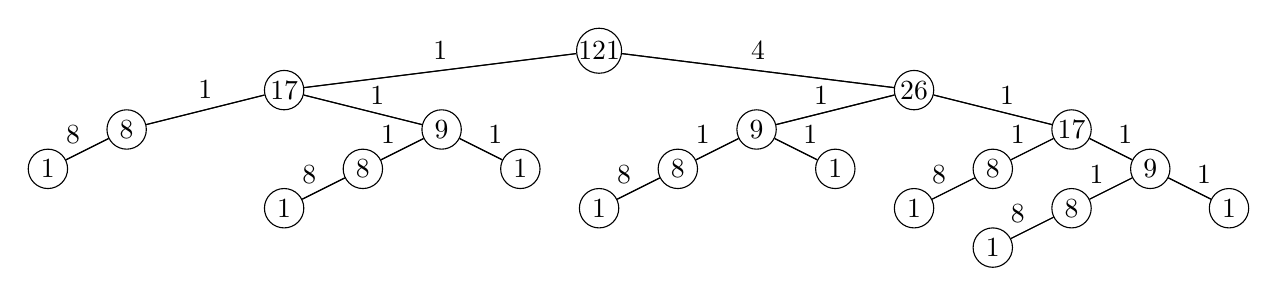
\begin{tikzpicture}[
  level distance=5mm,
  every node/.style={circle, draw, minimum size=5mm, inner sep=0},
  level 1/.style={sibling distance=80mm},
  level 2/.style={sibling distance=40mm},
  level 3/.style={sibling distance=20mm},
  label style/.style={draw=none, fill=none}
]

% If you want labels on each node, this is how you do it:
% child {node [label={[label distance=1mm] 180:remainder}] {17}

\node (root) {121}
    child {node (l1) {17}
        child {node (ll2) {8}
            child {node (lll3) {1}}
            child[missing]
        }
        child {node (lr2) {9}
            child {node (lrl3) {8}
                child {node (lrll4) {1}}
                child[missing]
            }
            child {node (lrr3) {1}}
        }
    }
    child {node (r1) {26}
        child {node (rl2) {9}
            child {node (rll3) {8}
                child {node (rlll4) {1}}
                child[missing]
            }
            child {node (rlr3) {1}}
        }
        child {node (rr2) {17}
            child {node (rrl3) {8}
                child {node (rrll4) {1}}
                child[missing]
            }
            child {node (rrr3) {9}
                child {node (rrrl4) {8}
                    child {node (rrrll5) {1}}
                    child[missing]
                }
                child {node (rrrr4) {1}}
            }
        }
    };

\draw (root) -- node [above, draw=none] {1} (l1);
\draw (root) -- node [above, draw=none] {4} (r1);

\draw (l1) -- node [above, draw=none] {1} (ll2);
\draw (l1) -- node [above right, draw=none] {1} (lr2);

\draw (r1) -- node [above left, draw=none] {1} (rl2);
\draw (r1) -- node [above right, draw=none] {1} (rr2);

\draw (ll2) -- node [above left, draw=none] {8} (lll3);

\draw (lr2) -- node [above left, draw=none] {1} (lrl3);
\draw (lr2) -- node [above right, draw=none] {1} (lrr3);

\draw (lrl3) -- node [above left, draw=none] {8} (lrll4);

\draw (rl2) -- node [above left, draw=none] {1} (rll3);
\draw (rl2) -- node [above right, draw=none] {1} (rlr3);

\draw (rll3) -- node [above left, draw=none] {8} (rlll4);

\draw (rr2) -- node [above left, draw=none] {1} (rrl3);
\draw (rr2) -- node [above right, draw=none] {1} (rrr3);

\draw (rrl3) -- node [above left, draw=none] {8} (rrll4);

\draw (rrr3) -- node [above left, draw=none] {1} (rrrl4);
\draw (rrr3) -- node [above right, draw=none] {1} (rrrr4);

\draw (rrrl4) -- node [above left, draw=none] {8} (rrrll5);

\end{tikzpicture}
\caption{\begin{minipage}{\linewidth} Vertical binary tree representation of groupings for $121 = 26 \cdot 4 + 17$. The numbers next to the lines denote the number of duplicate nodes/connections.
\end{minipage}}
\end{figure}

\subsection*{Summary}
This early logic of splitting quantities into equal parts—what we’ve termed group-splitting—may have seeded the more general and abstract idea of \textit{subdivision}. While group-splitting refers to a physical and perceptual behavior of repeatedly trying to split groups evenly, subdivision generalizes this behavior into the recursive reduction of quantities using smaller quantities. In this framing, group-splitting reflects an embodied response to imbalance—leftovers serve as perceptual prompts to continue splitting until all groups are even. It is this recursive tendency, grounded in physical interaction and visual perception, that underpins the intuitive origin of the Euclidean algorithm. It likely emerged not as a tool for computing the greatest common divisor (GCD), but from a more primitive compulsion to resolve imbalance —a perceptual drive that, through recursive action, gradually yielded an efficient method for subdivision.

\newpage

\section{From Even Grouping to Recursive Subdivision}
Once the behavior of recursively splitting leftovers into even groups became regular and repeatable, it may have prompted more structured reflection. In this section, we examine three natural ways people might have represented or refined this core process: (1) using fixed group sizes, (2) trying various splits by trial, and (3) discovering efficiency in reusing leftovers.

Each of these can be seen not as separate stages in a historical timeline, but as cognitive frames through which the same embodied behavior was interpreted, organized, and, eventually, formalized, into what we know today as the Euclidean algorithm.

\subsection{Fixed Group Sizes (Uniform Splitting)}
A common practice in early material cultures was to use fixed units—e.g., cubit rods, feet, spans—to measure or split things. In such contexts, people might have attempted to use a single, uniform group size across different quantities:

\begin{align*}
26 &= 3 \cdot 8 + 2, \\
17 &= 3 \cdot 5 + 2.
\end{align*}

This fixed-split approach simplifies comparison but often leaves many leftovers. The presence of multiple non-zero remainders becomes cognitively taxing, prompting interest in more efficient alternatives.

\subsection{Trial-and-Error Splitting}
In the absence of a fixed unit, a curious or pragmatic mind might experiment: what happens if I try splitting this group into 9s? Or 12s? This exploratory logic mirrors practices like laying stones of various sizes and adjusting as one goes. As seen below:

\begin{align*}
26 &= 16 \cdot 1 + 10, \\
17 &= 12 \cdot 1 + 5, \\
16 &= 12 \cdot 1 + 4, \\
10 &= 8 \cdot 1 + 2, \quad \text{and so on.}
\end{align*}

Though flexible, this approach generates many new quantities, for which the tracking/accounting quickly becomes untenable.

\subsection{Recursive Reuse of Leftovers (Efficient Splitting)}
Eventually, people may have realized a cleaner approach: reuse the leftover group to split the previous group. If a group of 17 remains after splitting 121 into 26s, try using 17 to split 26 (and the 17 itself, i.e., $17 = 17 \cdot 1  + 0$). Then, reuse the new remainder, and so on:

\begin{align*}
121 &= 26 \cdot 4 + 17, \\
26 &= 17 \cdot 1 + 9, \quad (17 = 17 \cdot 1 + 0) \\
17 &= 9 \cdot 1 + 8, \qquad (9 = 9 \cdot 1 + 0) \\
9 &= 8 \cdot 1 + 1, \qquad (8 = 8 \cdot 1 + 0) \\
8 &= 1 \cdot 8 + 0 \qquad (1 = 1 \cdot 1 + 0).
\end{align*}

Each leftover becomes the new \textit{splitter}, so the process naturally terminates when a split is even (i.e., has a remainder zero)---this is the Euclidean algorithm. So, rather than generating many arbitrary new split sizes, the recursive reuse method of the Euclidean algorithm leads to a minimal chain of quantities in a way that's efficient, structured, and cognitively economical.

\subsection*{Summary}
All three approaches—fixed splitting, trial splitting, and recursive reuse—can be seen as \textit{reinterpretations} of one core behavior: \textbf{trying to form \textit{even} groups}. What differs is the level of abstraction and structure. In this light, the Euclidean algorithm is not an abstract invention imposed upon nature; it is a refinement of a natural, embodied logic: when things don’t divide evenly, we split them evenly, one way o another, again and again, until they do (if they do).

\section{Conclusion}
The Euclidean algorithm, in its most refined form, reveals a minimalist and abstract strategy: use the remainder to measure the previous divisor, and repeat until nothing remains. But at its roots, this behavior may have emerged not from abstraction, but from the embodied act of trying to make even groups.

This paper proposed that what we now call the Euclidean algorithm was likely seeded by a much more intuitive and visual experience: group-splitting. In its earliest forms, this might have looked like a builder noticing leftovers when stacking bricks, or a steward redistributing sacks to avoid waste. Each time a remainder appeared—each moment of visual imbalance—it prompted the natural next question: can the leftover itself be split evenly? Over time, these perceptual and tactile interactions may have taken on structure. Attempts at fixed groupings may have given way to trial splits. Eventually, the reuse of leftovers offered a strategy that was cognitively lean and materially efficient. This recursive reuse—driven by the logic of resolving imbalance—converged toward the minimal chain of divisions that characterizes the Euclidean algorithm. This narrative suggests that the Euclidean algorithm did not descend from the heavens of abstraction but grew from the ground up, rooted in physical behavior. Its power lies not only in its efficiency but in its origins: the impulse to resolve leftover bits, to make all groups even, to discover simplicity through imbalance.

By tracing this conceptual trajectory—from intuitive group-splitting to recursive reuse—we gain a richer appreciation of the algorithm’s structure and its possible cognitive beginnings. It reminds us that even our most celebrated mathematical procedures may originate in something as humble as splitting piles, counting stones, and responding to the quiet mathematics of imbalance.


\section{Suggested Readings and Historical Context}

The ideas and historical interpretations in this paper are informed by a range of classical and modern sources. For readers interested in the development of the Euclidean algorithm, the nature of ancient measurement, and the emergence of abstract reasoning from physical practices, the following texts provide useful background:

\begin{itemize}
    \item Eleanor Robson, \textit{Mathematics in Ancient Iraq: A Social History} (2008).
    \item Wilbur Knorr, \textit{The Evolution of the Euclidean Elements} (1975).
    \item Reviel Netz, \textit{The Shaping of Deduction in Greek Mathematics} (1999).
    \item Euclid, \textit{Elements}, especially Book VII (on number theory and common measure).
    \item Michael S. Mahoney, \textit{The Mathematical Career of Pierre de Fermat} (for historical framing of algorithms).
\end{itemize}

\end{document}
